\section{Auswertung}
\label{sec:Auswertung}

\begin{figure}
  \centering
  \includegraphics{build/plankonkav.pdf}
  \caption{Darstellung der Messwerte sowie einer gefitteten Ausgleichsfunktion für den
  Resonator aus einem flachen und einem sphärischen Spiegel.}
  \label{fig:plankonkav}
\end{figure}

\begin{figure}
  \centering
  \includegraphics{build/konkavkonkav.pdf}
  \caption{Darstellung der Messwerte sowie einer gefitteten Ausgleichsfunktion für den
  Resonator aus zwei sphärischen Spiegeln.}
  \label{fig:konkavkonkav}
\end{figure}

\begin{figure}
  \centering
  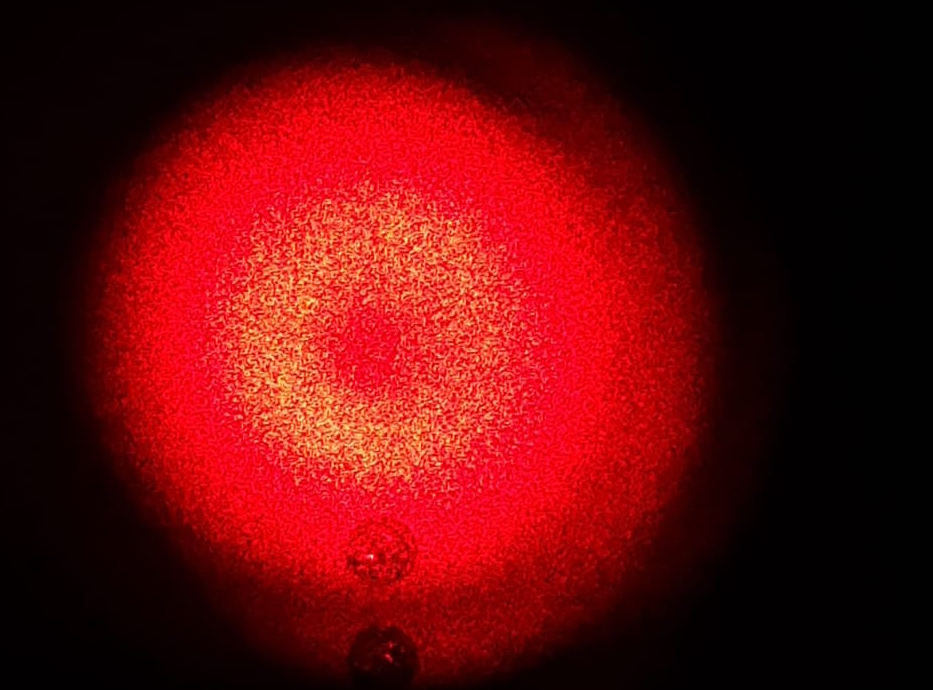
\includegraphics{build/tem00.pdf}
  \caption{Darstellung der Messwerte sowie einer gefitteten Ausgleichsfunktion für die $TEM_{0,0}$ Mode.}
  \label{fig:tem00}
\end{figure}

\begin{figure}
  \centering
  \includegraphics{build/tem01.pdf}
  \caption{Darstellung der Messwerte sowie einer gefitteten Ausgleichsfunktion für die $TEM_{0,1}$ Mode.}
  \label{fig:tem01}
\end{figure}


\begin{figure}
  \centering
  \includegraphics{build/polarisation.pdf}
  \caption{Darstellung der Messwerte sowie einer gefitteten Ausgleichsfunktion für die Intensität in
  Abhängigkeit vom Winkel des Polarisationsfilters.}
  \label{fig:polarisation}
\end{figure}
